\label{chap:benchmark_results}
This chapter describes benchmark characteristics like collection size and features and gives an overview of the performance of different Learning-to-Rank methods. Performance differences for a given Learning-to-Rank method are explained in terms of differences in benchmark characteristics. This chapter is concluded with a selection of Learning-to-Rank methods to include in the experiments.\\

Benchmarking datasets enable fair comparisons of ranking models over a fixed set of documents and queries. The approach of using fixed benchmarking datasets to compare the performance of Information Retrieval systems under equal circumstances has been the standard evaluation methodology in the Information Retrieval field since the release of the Cranfield collection \cite{Cleverdon1966}.
\section{Yahoo! Learning to Rank Challenge}
Yahoo's observation that all existing benchmark datasets were too small to draw reliable conclusions prompted Yahoo to release two internal datasets from Yahoo! search. Datasets used at commercial search engines are many times larger than available benchmark datasets. Yahoo! published a subset of their own commercial training data and launched a Learning-to-Rank competition based on this data. The Yahoo! Learning to Rank Challenge \cite{Chapelle2011a} is a public Learning-to-Rank competition which took place from March to May 2010, with the goal to promote the datasets and encourage the research community to develop new Learning-to-Rank algorithms.\\

The Yahoo! Learning to Rank Challenge consists of two tracks that uses the two datasets respectively: a standard Learning-to-Rank track and a transfer learning track where the goal was to learn a specialized ranking function that can be used for a small country by leveraging a larger training set of another country. For this experiment, I will only look at the standard Learning-to-Rank dataset, because transfer learning is a separate research area that is not included in this thesis.\\
\begin{table}[!h]
\begin{tabular}{l|lll}
 & Train & Validation & Test \\ 
 \hline
\# of queries & 19,994 & 2,994 & 6,983 \\ 
\# of documents & 473,134 & 71,083 & 165,660 \\ 
\# of features & 519 & 519 & 519 \\ 
\end{tabular}
\caption{Yahoo! Learning to Rank Challenge dataset characteristics, as described in the challenge overview paper \cite{Chapelle2011a}}
\label{tab:yahoo_characteristics}
\end{table}\\
Both \ac{nDCG} and \ac{ERR} are measured as performance metrics, but the final standings of the challenge were based on the \ac{ERR} values. Model validation on the Learning-to-Rank methods participating in the challenge is performed using a train/validation/test-set split following the characteristics shown in Table \ref{tab:yahoo_characteristics}. Competitors could train on the training set and get immediate feedback on their performance on the validation set. The test set performance is used to create the final standings and is only measured after the competition has ended to avoid overfitting on the test set. The large number of documents, queries and features compared to other benchmark datasets makes the Yahoo! Learning to Rank Challenge dataset interesting. Yahoo did not provide detailed feature descriptions to prevent competitors to get detailed insight in the characteristics of the Yahoo data collection and features used at Yahoo. Instead high level descriptions of feature categories are provided. The following categories of features are described in the challenge overview paper \cite{Chapelle2011a}:\\
\begin{description}
\item[Web graph]{Quality and popularity metrics of web documents, e.g. PageRank \cite{Page1999}}.
\item[Document statistics]{Basic document statistics such as the number of words and url characteristics.}
\item[Document classifier]{Results of various classifiers on the documents. These classifiers amongst others include: spam, adult, language, main topic, and quality classifiers.}
\item[Query]{Basic query statistics, such as the number of terms, query frequency, and click-through rate.}
\item[Text match]{Textual similarity metrics between query and document. Includes \ac{TF-IDF}, BM25 \cite{Robertson2009} and other metrics for different sections of the document.}
\item[Topical matching]{These features go beyond similarity at word level and compute similarity on topic level. For example by classifying both the document and the query in a large topical taxonomy.}
\item[Click]{Click-based user feedback.}
\item[External references]{Document meta-information such as Delicious\footnote{https://delicious.com/} tags}
\item[Time]{Document age and historical in- and outlink data that might help for time sensitive queries.}
\end{description}

\subsection{Results}
1055 teams send in at least one submission to the Yahoo! Learning to Rank challenge. The top eight participants of the Yahoo! Learning to Rank challenge all used decision trees combined with ensemble methods. The mainly used ensemble method within these top performers is boosting. The combination of boosting with decision tree learners is often called \acf{GBDT}. Figure \ref{fig:yahoo_results} shows the top five participants in the Yahoo! Learning to Rank Challenge in terms of ERR score.  Burges  \cite{Burges2011} created a linear combination ensemble of eight LambdaMART \cite{Burges2010}, two LambdaRank and two Logistic Regression models. Gottschalk and Vogel used a combination of RandomForest models and \ac{GBDT} models. Pavlov and Brunk used a regression based model using the BagBoo \cite{Pavlov2010} ensemble technique, which combines bagging and boosting. Sorokina used a similar combination of bagging and boosting that is called Additive Groves \cite{Sorokina2007}.\\

The challenge overview paper \cite{Chapelle2011a} states as one of the lessons of the challenge that the simple baseline \ac{GBDT} model performed very well with a small performance gap to the complex ensemble submissions at the top of the table.\\

\begin{table}
\begin{tabular}{l|p{6.3cm}|l}
 & Authors & ERR \\
 \hline 
1 & Burges et al. (Microsoft Research) & 0.46861 \\ 
2 & Gottschalk (Activision Blizzard) \& Vogel (Data Mining Solutions) & 0.46786 \\ 
3 & Parakhin (Microsoft) & 0.46695 \\ 
4 & Pavlov \& Brunk (Yandex Labs) & 0.46678 \\ 
5 & Sorokina (Yandex Labs) & 0.46616 \\ 
\end{tabular}
\caption{Final standings of the Yahoo! Learning to Rank Challenge, as presented in the challenge overview paper \cite{Chapelle2011a}}
\label{fig:yahoo_results}
\end{table}

Although the winning \ac{GBDT} models performs very well in terms of \ac{nDCG} their high complexity makes them unsuitable to use in production. The winning models take weeks to train and are very slow during query evaluation. An exception in training time is the BagBoo \cite{Pavlov2010} method used by Pavlov \& Brunk. The bagging component of the BagBoo method enables it to achieve high scalability through parallelism. Pavlov et al. \cite{Pavlov2010} managed to train half a million trees on 200 nodes in 2 hours.
\section{Yandex Internet Mathematics competition}

\subsection{Results}
The Yandex Internet Mathematics competition was won by Pavlov et al. \cite{Pavlov2010} with the BagBoo method.


\section{LETOR}
The LETOR benchmark set was first released by Microsoft Research Asia in April 2007 \cite{Liu2007b} to solve the absence of a experimental platform for Learning-to-Rank at that time. LETOR has been updated several times since: LETOR 2.0 was released at the end of 2007, LETOR 3.0 in December 2008 and LETOR 4.0 in July 2009.\\

\subsection{LETOR 3.0}
The LETOR 3.0 benchmark collection \cite{Qin2010} as released in 2007 contained two data sets: the OHSUMED collection and the .gov collection. The OHSUMED collection is a subset of the medical publication database MEDLINE and contains medical publications from 270 journals that were published between 1987 and 1991. The .gov collection is a web crawl obtained in January 2002, which was used for the \ac{TREC} web track in 2003 and 2004. Tables \ref{tbl:features_gov} and \ref{tbl:features_ohsumed} in Appendix \ref{chap:appendix_a} provide the descriptions of the features of the .gov and the OHSUMED collections respectively.\\

Different query sets exists for the .gov corpus. Those query sets are categorized in the following categories \cite{Craswell2003}:
\begin{description}
\item[topic distillation (TD)]these queries involve finding relevant pages given a broad query. E.g., the query 'cotton industry' which is entered with the aim to find pages that provide information about the cotton industry.
\item[named page finding (NP)]in these queries the user asks for one specific page by name. E.g., the user queries for 'ADA Enforcement' to find the page $http://www.usdoj.gov/crt/ada/enforce.htm$.
\item[home page finding (HP)]these queries are similar to NP queries in that the user is looking for one specific page, but now this specific page is a homepage. E.g., the user queries for 'Tennessee Valley Authority' to find the homepage $http://www.tva.gov$.
\end{description}
With query sets available from both the \ac{TREC} 2003 and 2004 conferences there are six query sets in total: TD2003, TD2004, NP2003, NP2004, HP2003 and HP2004.\\

The evaluation metrics used are \ac{nDCG} and \ac{MAP}. The \emph{winning number} metric is defined as the number of other algorithms that it can beat over all of the seven datasets (six .gov sets + OHSUMED). The LETOR organisation implemented and evaluated several well-known Learning-to-Rank algorithms themselves and in addition gathers and publications and results of new algorithms evaluated on the LETOR benchmark. The baseline Learning-to-Rank algorithms evaluated by the organisation are:
\begin{description}
\item[pointwise]{\leavevmode
	\begin{itemize}
	\item Linear regression
	\end{itemize}}
\item[pairwise]{\leavevmode
	\begin{itemize}
	\item Rank\ac{SVM} \cite{Herbrich1999,Joachims2002}
	\item RankBoost \cite{Freund2003}
	\item FRank \cite{Tsai2007}
	\end{itemize}}
\item[listwise]{\leavevmode
	\begin{itemize}
	\item ListNet \cite{Cao2007}
	\item AdaRank-MAP \cite{Xu2007}
	\item AdaRank-nDCG \cite{Xu2007}
	\item \ac{SVM}$^{MAP}$ \cite{Yue2007} 
	\end{itemize}}
\end{description} 


\subsection{Results}
The LETOR paper \cite{Qin2010} describes the performance of the LETOR baseline methods. Figures \ref{fig:ndcg_winning_number} and \ref{fig:map_winning_number} show ListNet to be the best performing baseline in terms of winning number on both \ac{nDCG} and \ac{MAP}. The LETOR website lists\footnote{http://research.microsoft.com/en-us/um/beijing/projects/letor/letor3baseline.aspx} a few algorithms that have since been evaluated on the LETOR benchmark collection.\\

\begin{figure}[!h]
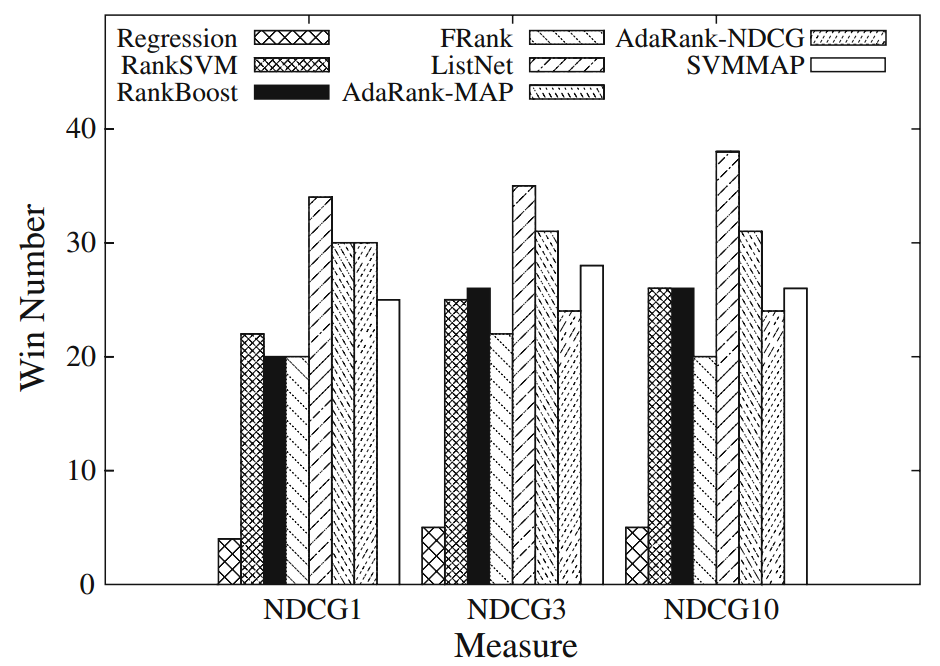
\includegraphics[scale=0.30]{gfx/ndcg_winning_number}
\caption{Comparison across the seven datasets in LETOR by \acs{nDCG}, obtained from Qin et al. \cite{Qin2010}}
\label{fig:ndcg_winning_number}
\end{figure}

\begin{figure}[!h]
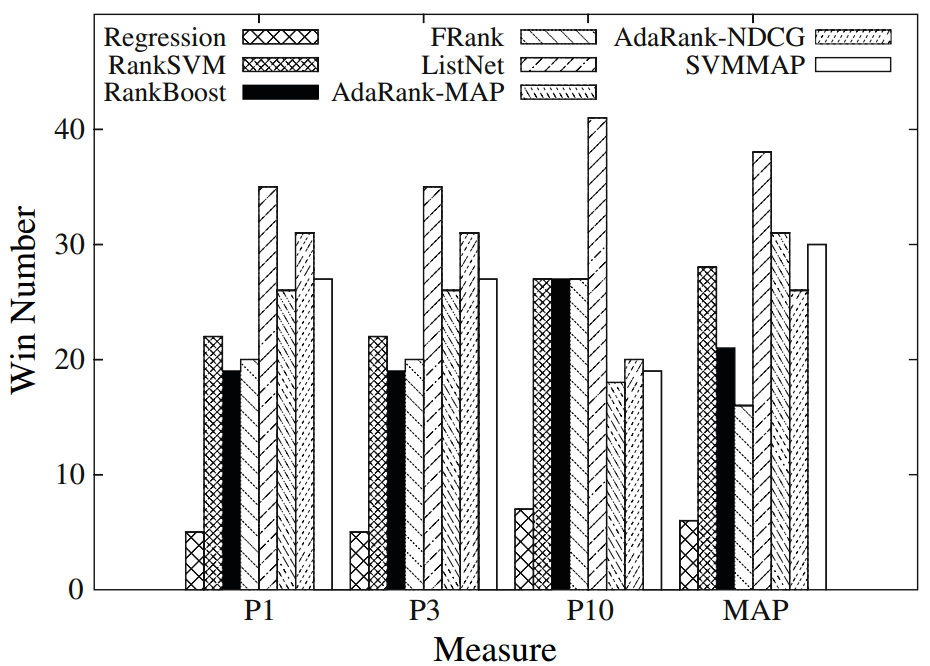
\includegraphics[scale=0.30]{gfx/map_winning_number}
\caption{Comparison across the seven datasets in LETOR by \acs{MAP}, obtained from Qin et al. \cite{Qin2010}}
\label{fig:map_winning_number}
\end{figure}

I will describe the performance of the algorithms that were evaluated by the LETOR team on LETOR 3.0 after publication of the LETOR paper by Qin et al. \cite{Qin2010}, as listed on the LETOR website\footnotemark[2] by comparing their performance with the ListNet baseline. We will consider those methods to be better than ListNet when they beat the ListNet baseline in at least four of the seven datasets in \ac{nDCG} value. Note that this does not necessarily imply that these methods would have scored a higher \ac{nDCG} winning number than ListNet. Table \ref{tbl:LETOR_ListNet} shows the ListNet performance on the seven LETOR datasets in terms of \ac{nDCG}@10 and \ac{MAP}.
\begin{table}
\begin{tabular}{l|ll}
 & \ac{nDCG}@10 & \ac{MAP} \\ 
 \hline
TD2003 & 0.348 & 0.2753 \\ 
TD2004 & 0.317 & 0.2231 \\ 
NP2003 & 0.801 & 0.6895 \\ 
NP2004 & 0.812 & 0.6720 \\ 
HP2003 & 0.837 & 0.7659 \\ 
HP2004 & 0.784 & 0.6899 \\ 
OHSUMED & 0.441 & 0.4457 \\ 
\end{tabular}
\caption{Performance of ListNet on LETOR 3.0}
\label{tbl:LETOR_ListNet}
\end{table}

Since LETOR is arguably the most well-known benchmark collection in the field, it is conceivable that creators of new Learning-to-Rank methods evaluate their new method on the LETOR collection to show how well their new method works. To create an overview of the performance of newer Learning-to-Rank methods on LETOR 3.0 we perform a forward reference search on the LETOR 3.0 paper \cite{Qin2010}. It should be noted that results of evaluations individually performed by the creator of the evaluated Learning-to-Rank method can not be regarded as equally reliable as the evaluations performed by the LETOR team. TODO: 307 citations, x evaluated a new Learning-to-Rank method on LETOR 3.0, x were usable. The unusable studies did test a new Learning-to-Rank method on one or more datasets of the LETOR collection, but 1 ) did not use a ranking metric used in LETOR (\ac{nDCG} or \ac{MAP}) or 2) did not list evaluation results at all.\\

\begin{table}
\begin{tabular}{l|p{1.2cm}p{1.2cm}p{1.2cm}p{1.4cm}||l}
 & \rotatebox{55}{Regression + L2 regulatisation} & \rotatebox{55}{Rank\ac{SVM}-Primal} &\rotatebox{55}{Rank\ac{SVM}-Struct} & \rotatebox{55}{SmoothRank} & \rotatebox{55}{ListNet} \\
 \hline
TD2003 & 0.3297 & 0.3571 & 0.3467 & 0.3367 & 0.348 \\ 
TD2004 & 0.2832 & 0.2913 & 0.3090 & 0.3343 & 0.317 \\ 
NP2003 & 0.8025 & 0.7894 & 0.7955 & 0.7986 & 0.801 \\ 
NP2004 & 0.8040 & 0.7950 & 0.7977 & 0.8075 & 0.812 \\ 
HP2003 & 0.8216 & 0.8180 & 0.8162 & 0.8325 & 0.837 \\ 
HP2004 & 0.7188 & 0.7720 & 0.7666 & 0.8221 & 0.784 \\ 
OHSUMED & 0.4436 & 0.4504 & 0.4523 & 0.4568 & 0.441 \\ 
\# winning datasets & 2 & 2 & 1 & 3 & - \\ 
\end{tabular}
\caption{\acs{nDCG}@10 comparison of algorithms recently evaluated on LETOR 3.0 with the ListNet baselines}
\label{tbl:LETOR_recently_added}
\end{table}

\subsection{LETOR 4.0}
The LETOR 4.0 benchmark collection\footnote{http://http://research.microsoft.com/en-us/um/beijing/projects/letor/} consists of the Gov-2 document collection and two query datasets from the Million Query Track at \ac{TREC} 2007 (MQ2007) and \ac{TREC} 2008 (MQ2008). LETOR 4.0 consists of a semi-supervised ranking task, a rank aggregation task and a listwise ranking task next to the supervised ranking task. Table \ref{tab:letor4_characteristics} shows the collection characteristics in number of queries, documents and features for LETOR 4.0. Evaluation on this collection is performed using a five-fold cross-validation, where partitioning of the data into folds was performed beforehand by the creators of the MQ2007 and MQ2008 datasets. Documents in the dataset were 

\begin{table}
\begin{tabular}{l|ll}
 Dataset & MQ2007 & MQ2008 \\ 
 \hline
 Queries & 1692 & 784 \\ 
 Documents & 69,622 & 15,211 \\
 Features & 46 & 46 \\
\end{tabular}
\caption{Characteristics of the LETOR 4.0 collection}
\label{tab:letor4_characteristics}
\end{table}
\subsubsection{Results}
Rank\ac{SVM}-Struct, ListNet, AdaRank-\ac{nDCG}, AdaRank-\ac{MAP} and RankBoost were used as baseline models on the LETOR 4.0 dataset and were implemented and evaluated by the publishers of LETOR 4.0. Table \ref{tab:letor4_baseline_results} shows the performance of those baseline models on the LETOR 4.0 benchmark collection.\\

\begin{table}
\begin{tabular}{l|lll}
Model & Dataset & Mean \ac{nDCG} & \ac{nDCG}@10 \\ 
\hline
Rank\ac{SVM}-Struct & MQ2007 & 0.4966 & 0.4439 \\ 
 & MQ2008 & 0.4832 & 0.2279 \\ 
\hline
ListNet & MQ2007 & 0.4988 & 0.4440 \\ 
 & MQ2008 & 0.4914 & 0.2303 \\ 
\hline
AdaRank-\ac{nDCG} & MQ2007 & 0.4914 & 0.4369 \\ 
 & MQ2008 & 0.4950 & 0.2307 \\ 
\hline
AdaRank-\ac{MAP} & MQ2007 & 0.4891 & 0.4335 \\ 
 & MQ2008 & 0.4915 & 0.2288 \\ 
\hline
RankBoost & MQ2007 & 0.5003 & 0.4464 \\ 
 & MQ2008 & 0.4850 & 0.2255 \\ 
\end{tabular}
\caption{Comparison of LETOR 4.0 baseline models}
\label{tab:letor4_baseline_results}
\end{table}

BoostedTree model \cite{Kocsis2013} showed an \ac{nDCG} of 0.5071 on the MQ2007 dataset and thereby beat all baseline models.

\section{MSLR-WEB10k/MSLR-WEB30k}
Contrary to the Yahoo! Learning to Rank Challenge dataset, the MSLR-WEB30k provides detailed feature descriptions. The MSLR-WEB30k dataset however contains no proprietary features but only features that are commonly used in the research community.
\subsection{Results}

\section{Selecting Learning-to-Rank methods}
The accuracies of the Learning-to-Rank methods described in the preceding sections must only be compared within the benchmark and not between benchmarks for the following reasons:
\begin{enumerate}
\item Differences in feature sets between data sets detract from fair comparison
\item Although the \ac{nDCG} definition is unambiguous, Busa-Fekete et al. \cite{Busa-Fekete2012} found that \ac{nDCG} evaluation tools of benchmark data sets produced different scores
\end{enumerate}

\section{Other datasets}
\subsection{WCL2R}
The WCL2R collection, released by Alc{\^a}ntara et al \cite{Alcantara2010}, contains of two datasets from the Chilean search engine TodoCL\footnote{www.todocl.cl}. Both datasets contain approximately 3 million documents. WCL2R is the only benchmark collection known that provides click-through data on user level. The collection contains 277,095 queries and logs of in total 1,5 million clicks by 16,829 users. The WCL2R paper provides evaluation results for the well-known Rank\ac{SVM} \cite{Herbrich1999,Joachims2002} and RankBoost \cite{Freund2003} algorithms. In addition two ranking methods developed at the same university of the WCL2R paper were evaluated: LAC \cite{Veloso2008} and a ranking algorithm based on \ac{GP} \cite{DeAlmeida2007}. Table \ref{tab:results_WCL2R} shows the performance of those algorithms on the WCL2R collection. No evaluations of other algorithms on the WCL2R collection are known.

\begin{table}
\begin{tabular}{l|lll|lll}
 &  & FS &  &  & NC &  \\ 
\hline
Algorithm & @1 & @3 & @10 & @1 & @3 & @10 \\ 
\hline
RankSVM & 0.314 & 0.353 & 0.395 & 0.265 & 0.301 & 0.339 \\ 
LAC & 0.296 & 0.360 & 0.403 & 0.244 & 0.266 & 0.315 \\ 
GP & 0.288 & 0.344 & 0.396 & 0.221 & 0.262 & 0.318 \\ 
RankBoost & 0.295 & 0.328 & 0.375 & 0.247 & 0.264 & 0.305 \\ 
\end{tabular}
\caption{\acs{nDCG} results of baseline methods on the WCL2R collection, obtained from \cite{Alcantara2010}}
\label{tab:results_WCL2R}
\end{table}